\documentclass[aspectratio=43]{beamer}
\usetheme{Pittsburgh}
\usepackage[utf8]{inputenc}
\usepackage[german]{babel}
\usepackage{amsmath}
\usepackage{amsfonts}
\usepackage{amssymb}
\usepackage{graphicx}
\usepackage{multicol}
\usepackage{wrapfig}
\usepackage{hyperref}
\usepackage{minted}

\author{Jonas Betzendahl}
\title{Hilberts Albtraum}

\beamertemplatenavigationsymbolsempty 

% For Footnotes without markers on the slide
% https://tex.stackexchange.com/questions/30720/footnote-without-a-marker
\newcommand\blfootnote[1]{%
  \begingroup
  \renewcommand\thefootnote{}\footnote{#1}%
  \addtocounter{footnote}{-1}%
  \endgroup
}

\begin{document}

%------------------------------------------------------------------------------------
\section{Introduction}

\begin{frame}
\begin{center}
\Large \glqq Hilberts Albtraum\grqq
\normalsize 

(The answer may \textit{not} be out there!)
\bigskip\bigskip

\Large \texttt{@jbetzend}
\smallskip

\href{https://twitter.com/jbetzend}{
\includegraphics[scale=0.125]{images/twitter_logo.png}}
\href{https://github.com/jbetzend}{
\includegraphics[scale=0.125]{images/github_logo.png}}
\href{https://whispeer.de/en/user/jbetzend}{
\includegraphics[scale=0.125]{images/whispeer_logo.png}}
\end{center}
\end{frame}

%------------------------------------------------------------------------------------

\begin{frame}
\frametitle{Mein Thema}

\begin{center}
\emph{Wie kann ich einem Computer beibringen,\\ mit mathematischen Beweisen umzugehen?}
\bigskip\bigskip

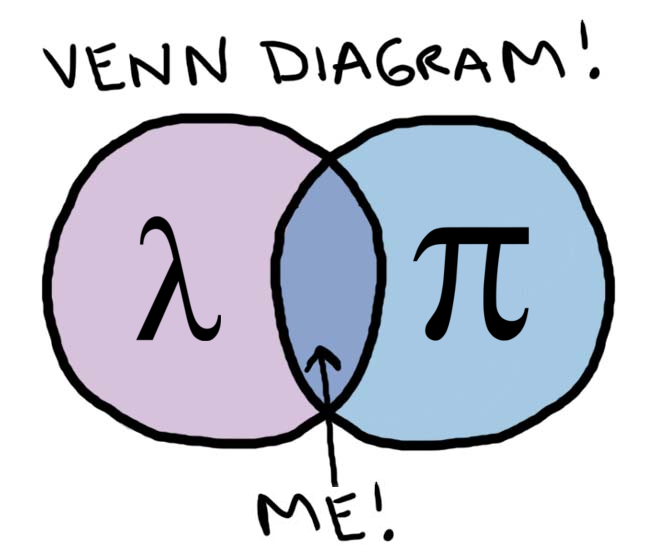
\includegraphics[width=0.45\textwidth]{images/venn-diagram.jpg} 
\end{center}

\blfootnote{\glqq Venn Diagram\grqq\ by unknown artist, modified, Image under Fair Use}
\end{frame}

%------------------------------------------------------------------------------------

\begin{frame}
 
\vspace{40pt}

\begin{center}
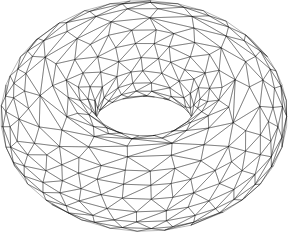
\includegraphics[scale=0.5]{images/torus.png}
\bigskip\bigskip

Mathematik ist eine Wissenschaft

\emph{fast} wie jede andere\dots
\end{center}

\blfootnote{\href{https://openclipart.org/detail/277014/3d-torus-rotated-wireframe-2}{\glqq 3D Torus \dots\grqq\ by GDJ, \texttt{www.openclipart.org}}, licensed \texttt{CC-0}}

\end{frame}

%------------------------------------------------------------------------------------

\begin{frame}
\begin{quote}
    Math is the reverse of comedy. The anti-joke.\\
    We'll tell you the punchline first, then
    laboriously explain to you
    why it was the right punchline.
\end{quote}
\begin{center}
\textit{Joseph Maher}, College of Staten Island 
\end{center}

\end{frame}

%------------------------------------------------------------------------------------

\begin{frame}
\begin{center}
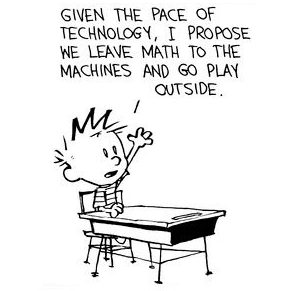
\includegraphics[scale=0.7]{images/go_play_outside.jpg} 
\end{center}
\blfootnote{\href{http://www.gocomics.com/calvinandhobbes/1992/11/25}{\glqq Calvin \& Hobbes, 25 NOV 1992\grqq\ by Bill Waterson, Image under Fair Use}}
\end{frame}

%------------------------------------------------------------------------------------

\begin{frame}
\frametitle{David Hilbert}

\begin{multicols}{2}

Mathematiker (1862-1943) aus Königsberg, bekannt für seine Grundlagenforschung und Problemsammlungen.
\bigskip

\emph{\underline{Hilberts Traum:}}\\\smallskip

Ein Computer, dem ich eine beliebige mathematische Aussage reichen kann und der mir sagt, ob sie stimmt. 

\columnbreak

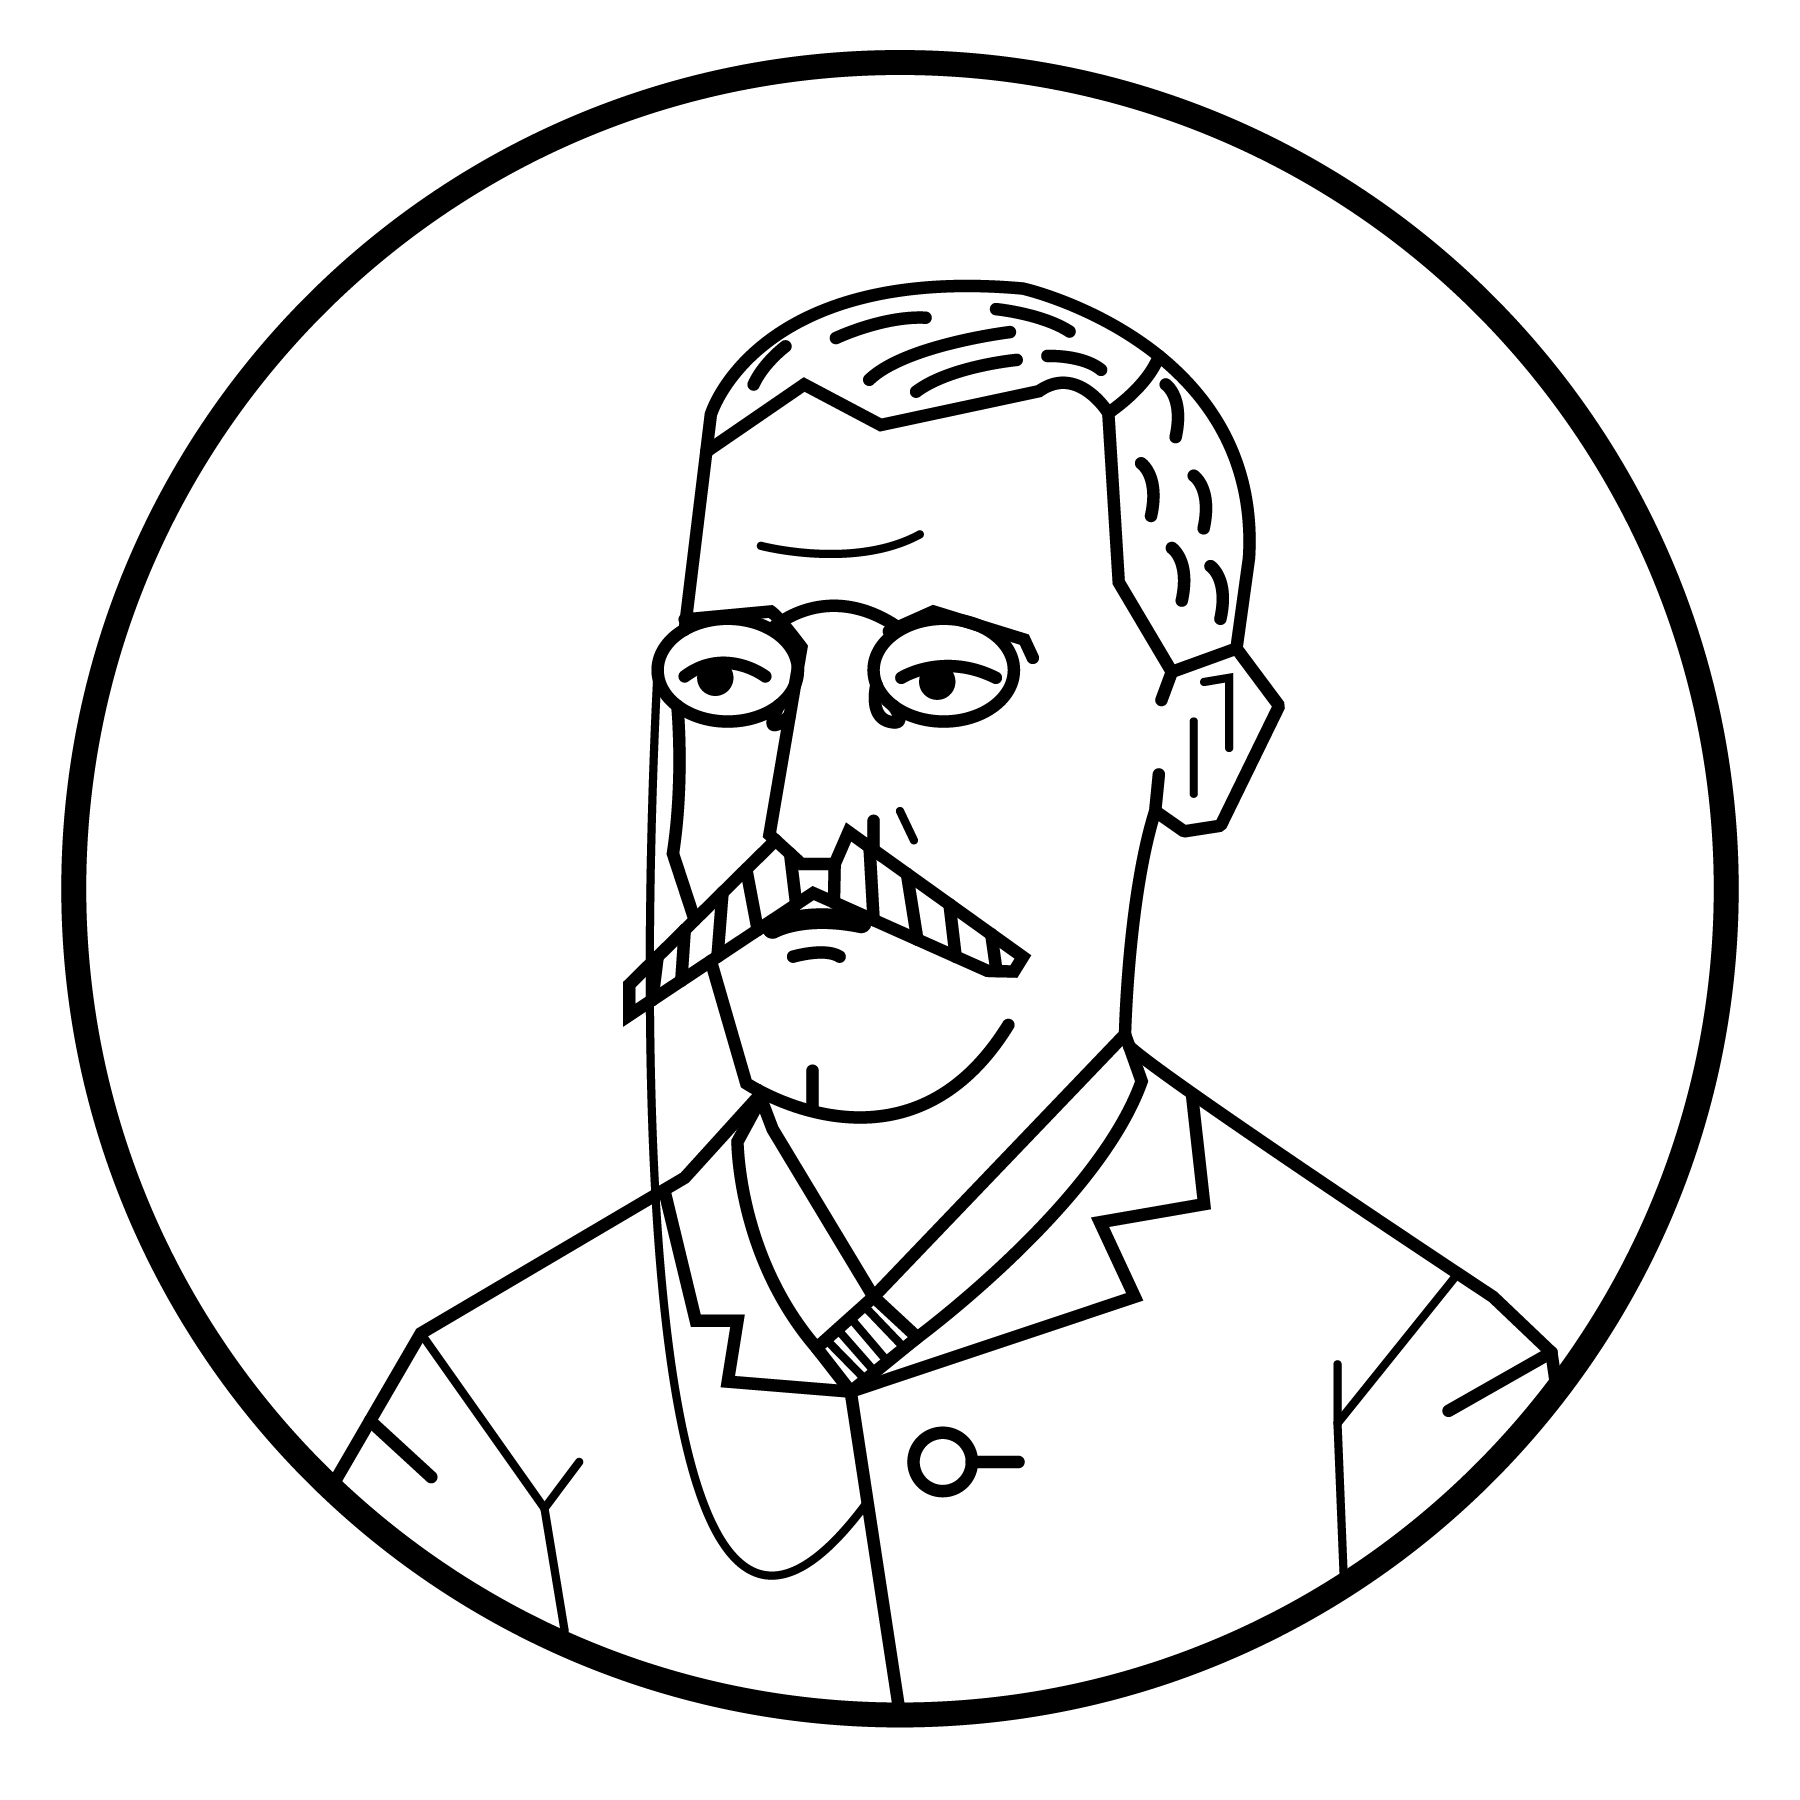
\includegraphics[scale=0.3]{images/hilbert-circle.png} 

\end{multicols}

\blfootnote{\glqq David Hilbert\grqq\ by Matthew Leadbeater, licensed \texttt{CC-BY-NC}, 2016}

\end{frame}

%------------------------------------------------------------------------------------

\begin{frame}
\vspace{20pt}
\begin{multicols}{2}

Das ist leicht zu schaffen, wenn wir das \emph{Halteproblem} lösen!
\smallskip

(z.B. durch Auflistung aller Folgerungen aus den Axiomen)
\bigskip

\emph{\underline{Halteproblem:}}\\

Gegeben nur den Quellcode und den Input eines Programms, sage vorher ob dieses Programm jemals \glqq fertig wird\grqq\ oder endlos weiter läuft.

\columnbreak

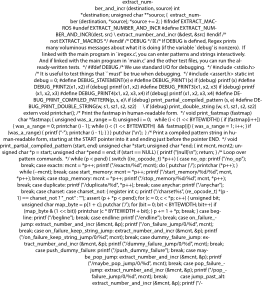
\includegraphics[scale=0.55]{images/CodeHeadText.png} 

\end{multicols}

\blfootnote{\href{https://openclipart.org/detail/274575/code-head-text}{\glqq Code Head Text\grqq\ by GDJ, \texttt{www.openclipart.org}}, licensed \texttt{CC-0}}

\end{frame}

%------------------------------------------------------------------------------------

\begin{frame}[fragile]

Manchmal ist es sehr leicht zu sehen, ob ein Programm jemals halten wird oder nicht:

\begin{framed}
\begin{minted}{haskell}
-- Dieses Programm hält quasi sofort
main :: IO ()
main = print $ plus (3,4)
  where
    plus :: (Int, Int) -> Int
    plus (x,y) = x + y
\end{minted}
%$
\end{framed}

\pause

\begin{framed}
\begin{minted}{haskell}
-- Dieses Programm läuft "für immer"
main :: IO ()
main = forever $ print "lol, infinite loop!"
\end{minted}
\end{framed}
%$

\end{frame}

%------------------------------------------------------------------------------------

\begin{frame}[fragile]

Manchmal ist es aber auch nahezu unmöglich!

\begin{framed}
\begin{minted}{haskell}
-- Nobody knows if this ever halts...
main :: IO ()
main = do let results = filter isPerfect [1,3..]
          case results of
            [] -> print " No odd perfect numbers!"
            _  -> print "Yes odd perfect numbers!"

divisors :: Int -> [Int]
divisors n = filter (\x -> n `rem` x == 0) [1..n]

isPerfect :: Int -> Bool
isPerfect n = (sum . divisors) n == n + n
\end{minted}
\end{framed}


\end{frame}


%------------------------------------------------------------------------------------

\begin{frame}
\frametitle{Alan Turing}

\begin{multicols}{2}

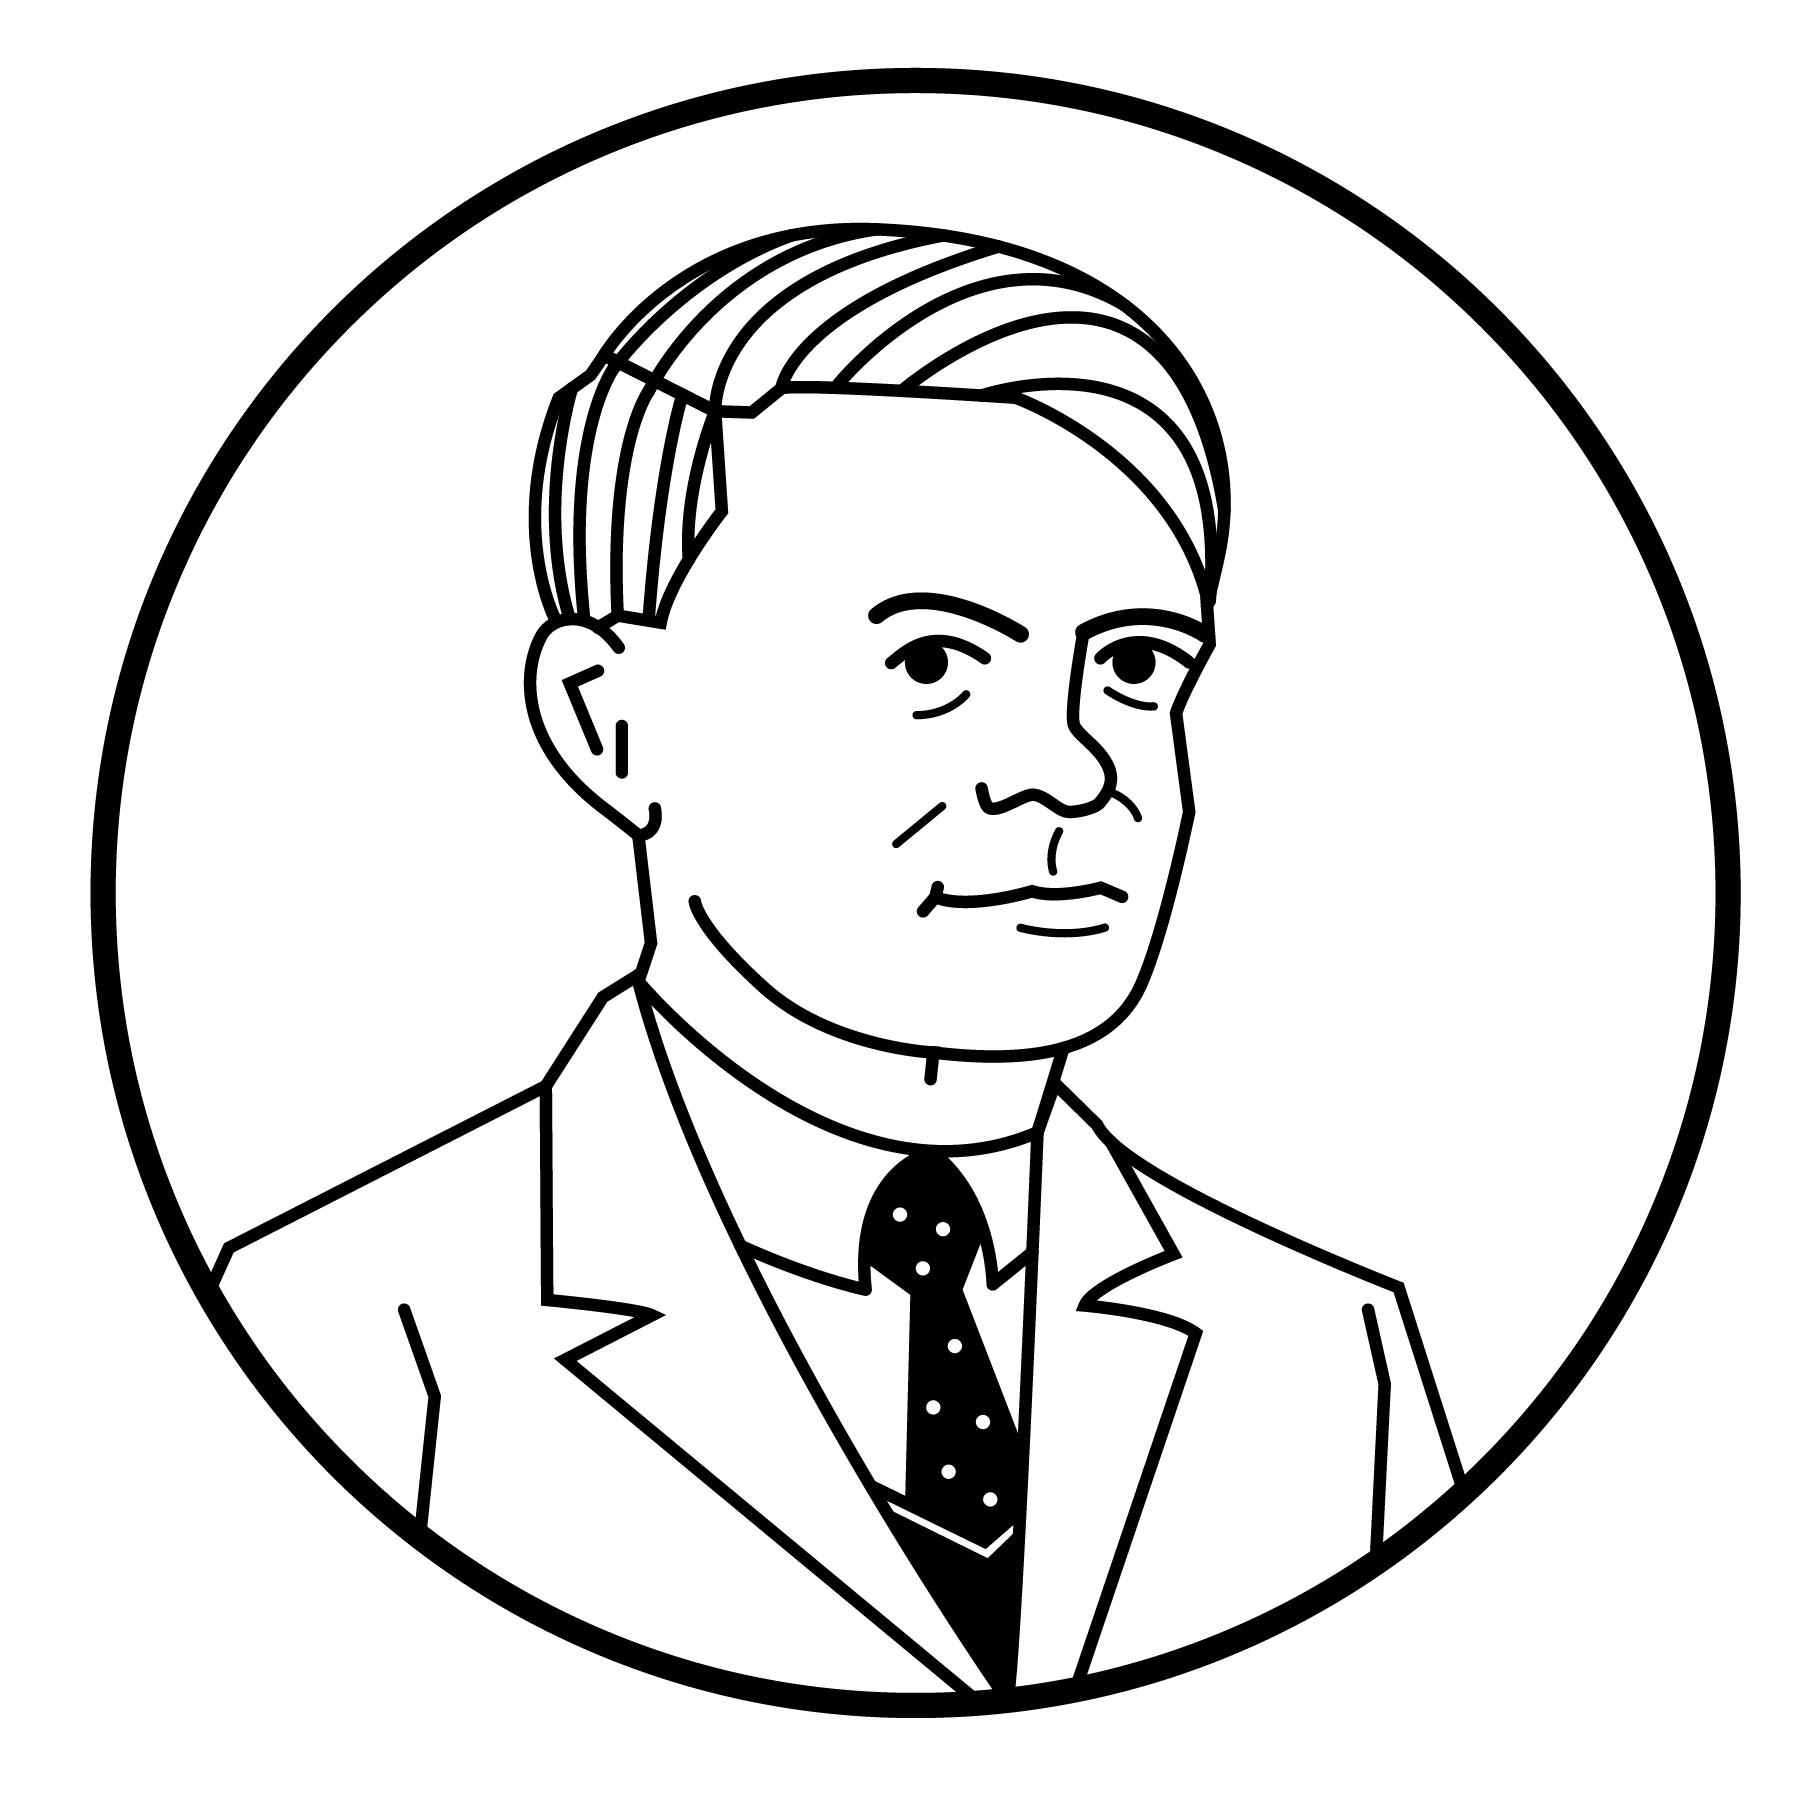
\includegraphics[scale=0.3]{images/turing-circle.png} 

\columnbreak

Mathematiker (1912-1954) aus London. Half in Bletchley Park, den dt. \emph{Enigma}-Code zu lösen.
\bigskip

Bewies in seiner Doktorarbeit, dass das Halteproblem \emph{nicht lösbar sein kann} (zumindest im allgemeinen Fall)!
\pause\bigskip

Aber nehmen wir mal an, es \emph{wäre lösbar}\dots

\end{multicols}

\blfootnote{\glqq Alan Turing\grqq\ by Matthew Leadbeater, licensed \texttt{CC-BY-NC}, 2016}
\end{frame}

%------------------------------------------------------------------------------------

\begin{frame}
\frametitle{Ein magisches Halte-Orakel (1)}
\begin{center}

\includegraphics[scale=1.4]{images/hat_alone.png} 
\end{center}
\end{frame}

%------------------------------------------------------------------------------------

\begin{frame}
\frametitle{Ein magisches Halte-Orakel (2)}
\begin{center}
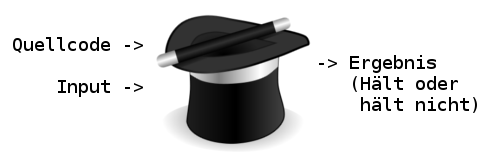
\includegraphics[scale=1.4]{images/erklaerung01.png} 
\end{center}
\end{frame}

%------------------------------------------------------------------------------------

\begin{frame}
\frametitle{Ein magisches Halte-Orakel (3)}
\begin{center}
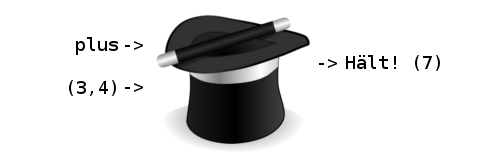
\includegraphics[scale=1.4]{images/erklaerung02.png} 
\end{center}
\end{frame}

%------------------------------------------------------------------------------------

\begin{frame}
\frametitle{Ein magisches Halte-Orakel (4)}
\begin{center}
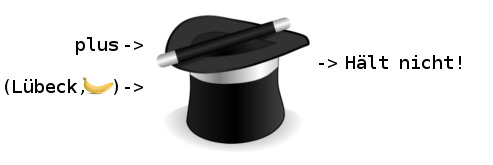
\includegraphics[scale=1.4]{images/erklaerung03.png} 
\end{center}
\end{frame}

%------------------------------------------------------------------------------------

\begin{frame}
\frametitle{Negierer (1)}
\begin{center}

\includegraphics[scale=1.4]{images/erklaerung04.png} 
\bigskip

Dazu kommt ein Negierer, der ein Haltergebnis umdreht!
\end{center}
\end{frame}

%------------------------------------------------------------------------------------

\begin{frame}
\frametitle{Negierer (2)}
\begin{center}
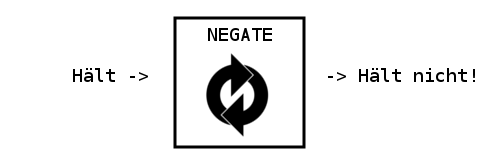
\includegraphics[scale=1.4]{images/erklaerung05.png}
\bigskip

Dazu kommt ein Negierer, der ein Haltergebnis umdreht!
\end{center}
\end{frame}

%------------------------------------------------------------------------------------

\begin{frame}
\frametitle{Negierer (3)}
\begin{center}
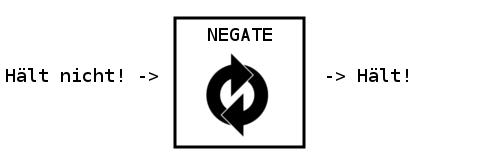
\includegraphics[scale=1.4]{images/erklaerung06.png}
\bigskip

Dazu kommt ein Negierer, der ein Haltergebnis umdreht!
\end{center}
\end{frame}

%------------------------------------------------------------------------------------

\begin{frame}
\frametitle{Duplizierer (1)}
\begin{center}

\includegraphics[scale=1.4]{images/copy_alone.png} 
\bigskip

Wir haben auch einen Duplizierer, der seine Eingabe verdoppelt!
\end{center}
\end{frame}

%------------------------------------------------------------------------------------

\begin{frame}
\frametitle{Duplizierer (2)}
\begin{center}
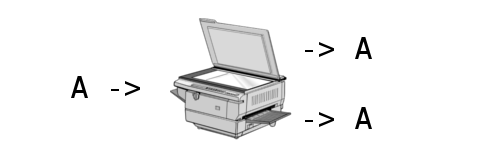
\includegraphics[scale=1.4]{images/erklaerung07.png}
\bigskip

Wir haben auch einen Duplizierer, der seine Eingabe verdoppelt!
\end{center}
\end{frame}

%------------------------------------------------------------------------------------

\begin{frame}
\frametitle{Duplizierer (3)}
\begin{center}
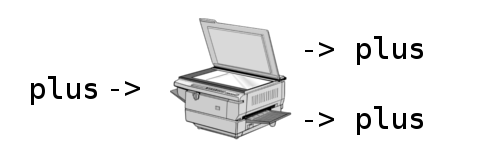
\includegraphics[scale=1.4]{images/erklaerung08.png}
\bigskip

Wir haben auch einen Duplizierer, der seine Eingabe verdoppelt!
\end{center}
\end{frame}

%------------------------------------------------------------------------------------

\begin{frame}
\frametitle{Unite and conquer! (1)}
\begin{center}
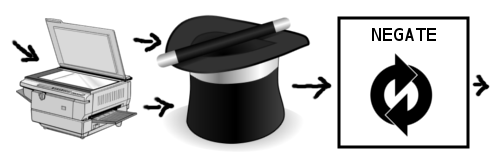
\includegraphics[scale=1.4]{images/complete.png} 
\bigskip

Sie ahnen es! Alles das können wir jetzt zusammen stecken!
\end{center}
\end{frame}

%------------------------------------------------------------------------------------

\begin{frame}
\frametitle{Unite and conquer! (2)}
\begin{center}
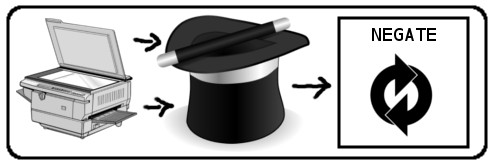
\includegraphics[scale=1.4]{images/complete_border.png} 
\bigskip

Insbesondere können wir diese Aneinanderreihung als \emph{eine Maschine} betrachen. Nennen wir sie \texttt{X}.
\end{center}
\end{frame}

%------------------------------------------------------------------------------------

\begin{frame}
\frametitle{Unite and conquer! (3)}
\begin{center}

\includegraphics[scale=1.4]{images/complete_border_filled.png} 
\bigskip

Insbesondere können wir diese Aneinanderreihung als \emph{eine Maschine} betrachen. Nennen wir sie \texttt{X}.
\end{center}
\end{frame}

%------------------------------------------------------------------------------------

\begin{frame}
\frametitle{Going Meta! (1)}
\begin{center}
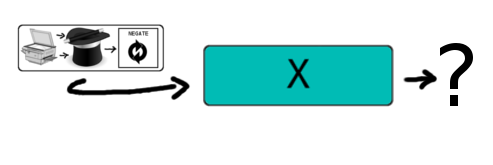
\includegraphics[scale=1.4]{images/input.png} 
\bigskip

Jetzt nur keine Panik bekommen!\\

Aber was passiert, wenn wir den Quellcode von \texttt{X} an \texttt{X} geben?
\end{center}
\end{frame}

%------------------------------------------------------------------------------------

\begin{frame}
\frametitle{Going Meta! (2)}

\begin{center}
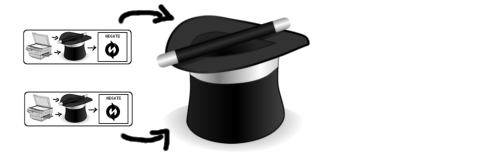
\includegraphics[scale=1.4]{images/input_hat_nothing.png} 
\bigskip

foo\\
bar
\end{center}
\end{frame}

%------------------------------------------------------------------------------------

\begin{frame}
\frametitle{Fall 1: Orakel sagt "Hält!"}

\begin{center}
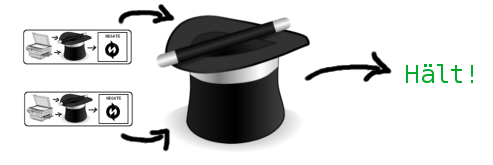
\includegraphics[scale=1.4]{images/input_hat_halts.png} 
\bigskip

foo\\
bar
\end{center}
\end{frame}

%------------------------------------------------------------------------------------

\begin{frame}
\frametitle{Fall 2: Orakel sagt "Hält nicht!"}

\begin{center}
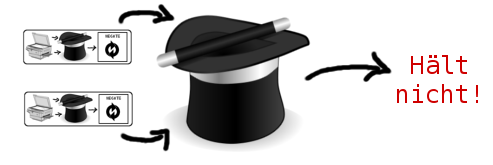
\includegraphics[scale=1.4]{images/input_hat_haltsnot.png} 
\bigskip

foo\\
bar
\end{center}
\end{frame}

%------------------------------------------------------------------------------------

\begin{frame}
\frametitle{Widerspruch}
\begin{center}
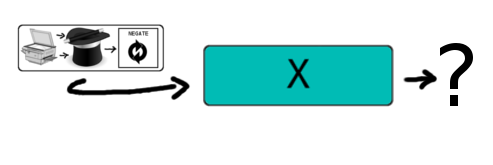
\includegraphics[scale=1.4]{images/input.png} 
\bigskip

Was bleibt uns von unserer erdachten magischen Maschine?\\
Jeder mögliche Weg führt zum Widerspruch!
\pause\bigskip

Damit ist bewiesen: so ein Orakel \emph{kann} es nicht geben!\\
Das Halteproblem ist (im Allgemeinen) unlösbar!
\end{center}
\end{frame}

%------------------------------------------------------------------------------------

\begin{frame}
\frametitle{Widerspruch}
\begin{center}
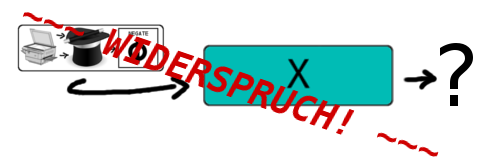
\includegraphics[scale=1.4]{images/input_contradiction.png} 
\bigskip

Was bleibt uns von unserer erdachten magischen Maschine?\\
Jeder mögliche Weg führt zum Widerspruch!
\bigskip

Damit ist bewiesen: so ein Orakel \emph{kann} es nicht geben!\\
Das Halteproblem ist (im Allgemeinen) unlösbar!
\end{center}
\end{frame}

%------------------------------------------------------------------------------------

\begin{frame}
\frametitle{Schlusswort}

\end{frame}
\end{document}